\subsection{Kiến trúc phần mềm}
Phần mềm được tổ chức thành năm thành phần, với \textbf{một ràng buộc kiến trúc bất biến} quyết định toàn bộ cách làm việc của đề tài.

\begin{table}[!htbp]
  \centering
  \caption{Các thành phần phần mềm và vai trò}
  \small
  \renewcommand{\arraystretch}{1.25}
  \begin{tabular}{>{\raggedright\arraybackslash}p{0.2043\textwidth}>{\raggedright\arraybackslash}p{0.7245\textwidth}}
    \toprule
    \textbf{Thành phần} & \textbf{Vai trò} \\
    \midrule
    Lớp lõi & Thuần C++, \textbf{không} phụ thuộc bất kỳ thư viện phần cứng nào. Chứa toàn bộ ba thuật toán, xử lý tín hiệu khí, hình học, quản lý nhiệm vụ và định dạng bản tin \\
    Firmware xe & Trình điều khiển phần cứng: động cơ, encoder, IMU, ADC, nút bấm, LED \\
    Firmware trạm thu & Nhận gói LoRa, kiểm tra checksum, in ra hai dạng, gửi lệnh lên xe \\
    Trình mô phỏng & Chạy trên máy tính, cung cấp một robot ảo cho lớp lõi \\
    Bộ kiểm thử tự động & 86 phép kiểm tra chạy trên máy tính, dùng lại robot ảo làm robot giả \\
    \bottomrule
  \end{tabular}
\end{table}
Bảng 4.1 liệt kê năm thành phần đó. \textbf{Ràng buộc kiến trúc:} lớp lõi chỉ giao tiếp với phần cứng thông qua một giao diện trừu tượng gồm các lệnh như ``đi tới'', ``quay'', ``đọc khí'', ``đã va chạm chưa''. Khi chạy trên xe, các lệnh đó nối vào động cơ và cảm biến thật. Khi chạy trên máy tính, chúng nối vào mô hình. Nhờ vậy \textbf{cùng một tệp mã nguồn thuật toán chạy được trên cả hai phía}, và \textbf{không tồn tại ``bản mô phỏng'' khác với ``bản thật''}. Đây là nền tảng cho toàn bộ tính hợp lệ của phần kết quả ở Chương 6.

Ba quy tắc phụ trợ đi kèm: hàm cập nhật của thuật toán \textbf{không được phép chặn} (không có lệnh chờ, không có vòng lặp bận), để vòng điều khiển 50 Hz luôn chạy đúng nhịp; ba thuật toán được cấp phát tĩnh chứ không dùng bộ nhớ động, để tránh phân mảnh bộ nhớ trong một chương trình chạy dài trên vi điều khiển; và \textbf{mọi hằng số của hệ thống nằm tập trung tại một tệp cấu hình duy nhất}, không rải rác trong mã.

\textbf{Xử lý cấu hình một encoder.} Như đã nêu ở mục 3.4, phần cứng chỉ có một encoder. Firmware xử lý theo ba bước: chỉ gắn ngắt cho encoder thực sự tồn tại; lấy quãng đường \textbf{trực tiếp} từ encoder trái thay vì lấy trung bình hai bên; và khi phát hiện hai bên đang được cấp lệnh ngược chiều nhau --- tức là xe đang quay tại chỗ --- thì đặt quãng đường tăng thêm bằng \textbf{không}. Cách xử lý này đúng cho cả cấu hình một lẫn hai encoder, nên nếu sau này lắp thêm encoder thứ hai thì chỉ cần đổi một hằng số cấu hình. Đồng thời, vì không thể suy góc quay từ hiệu hai encoder, MPU6050 trở thành \textbf{bắt buộc}: firmware chặn lệnh chạy và in cảnh báo nếu không tìm thấy nó.


\subsection{Chuỗi xử lý tín hiệu khí --- hai lớp dữ liệu tách biệt}
\begin{figure}[!p]
  \centering
  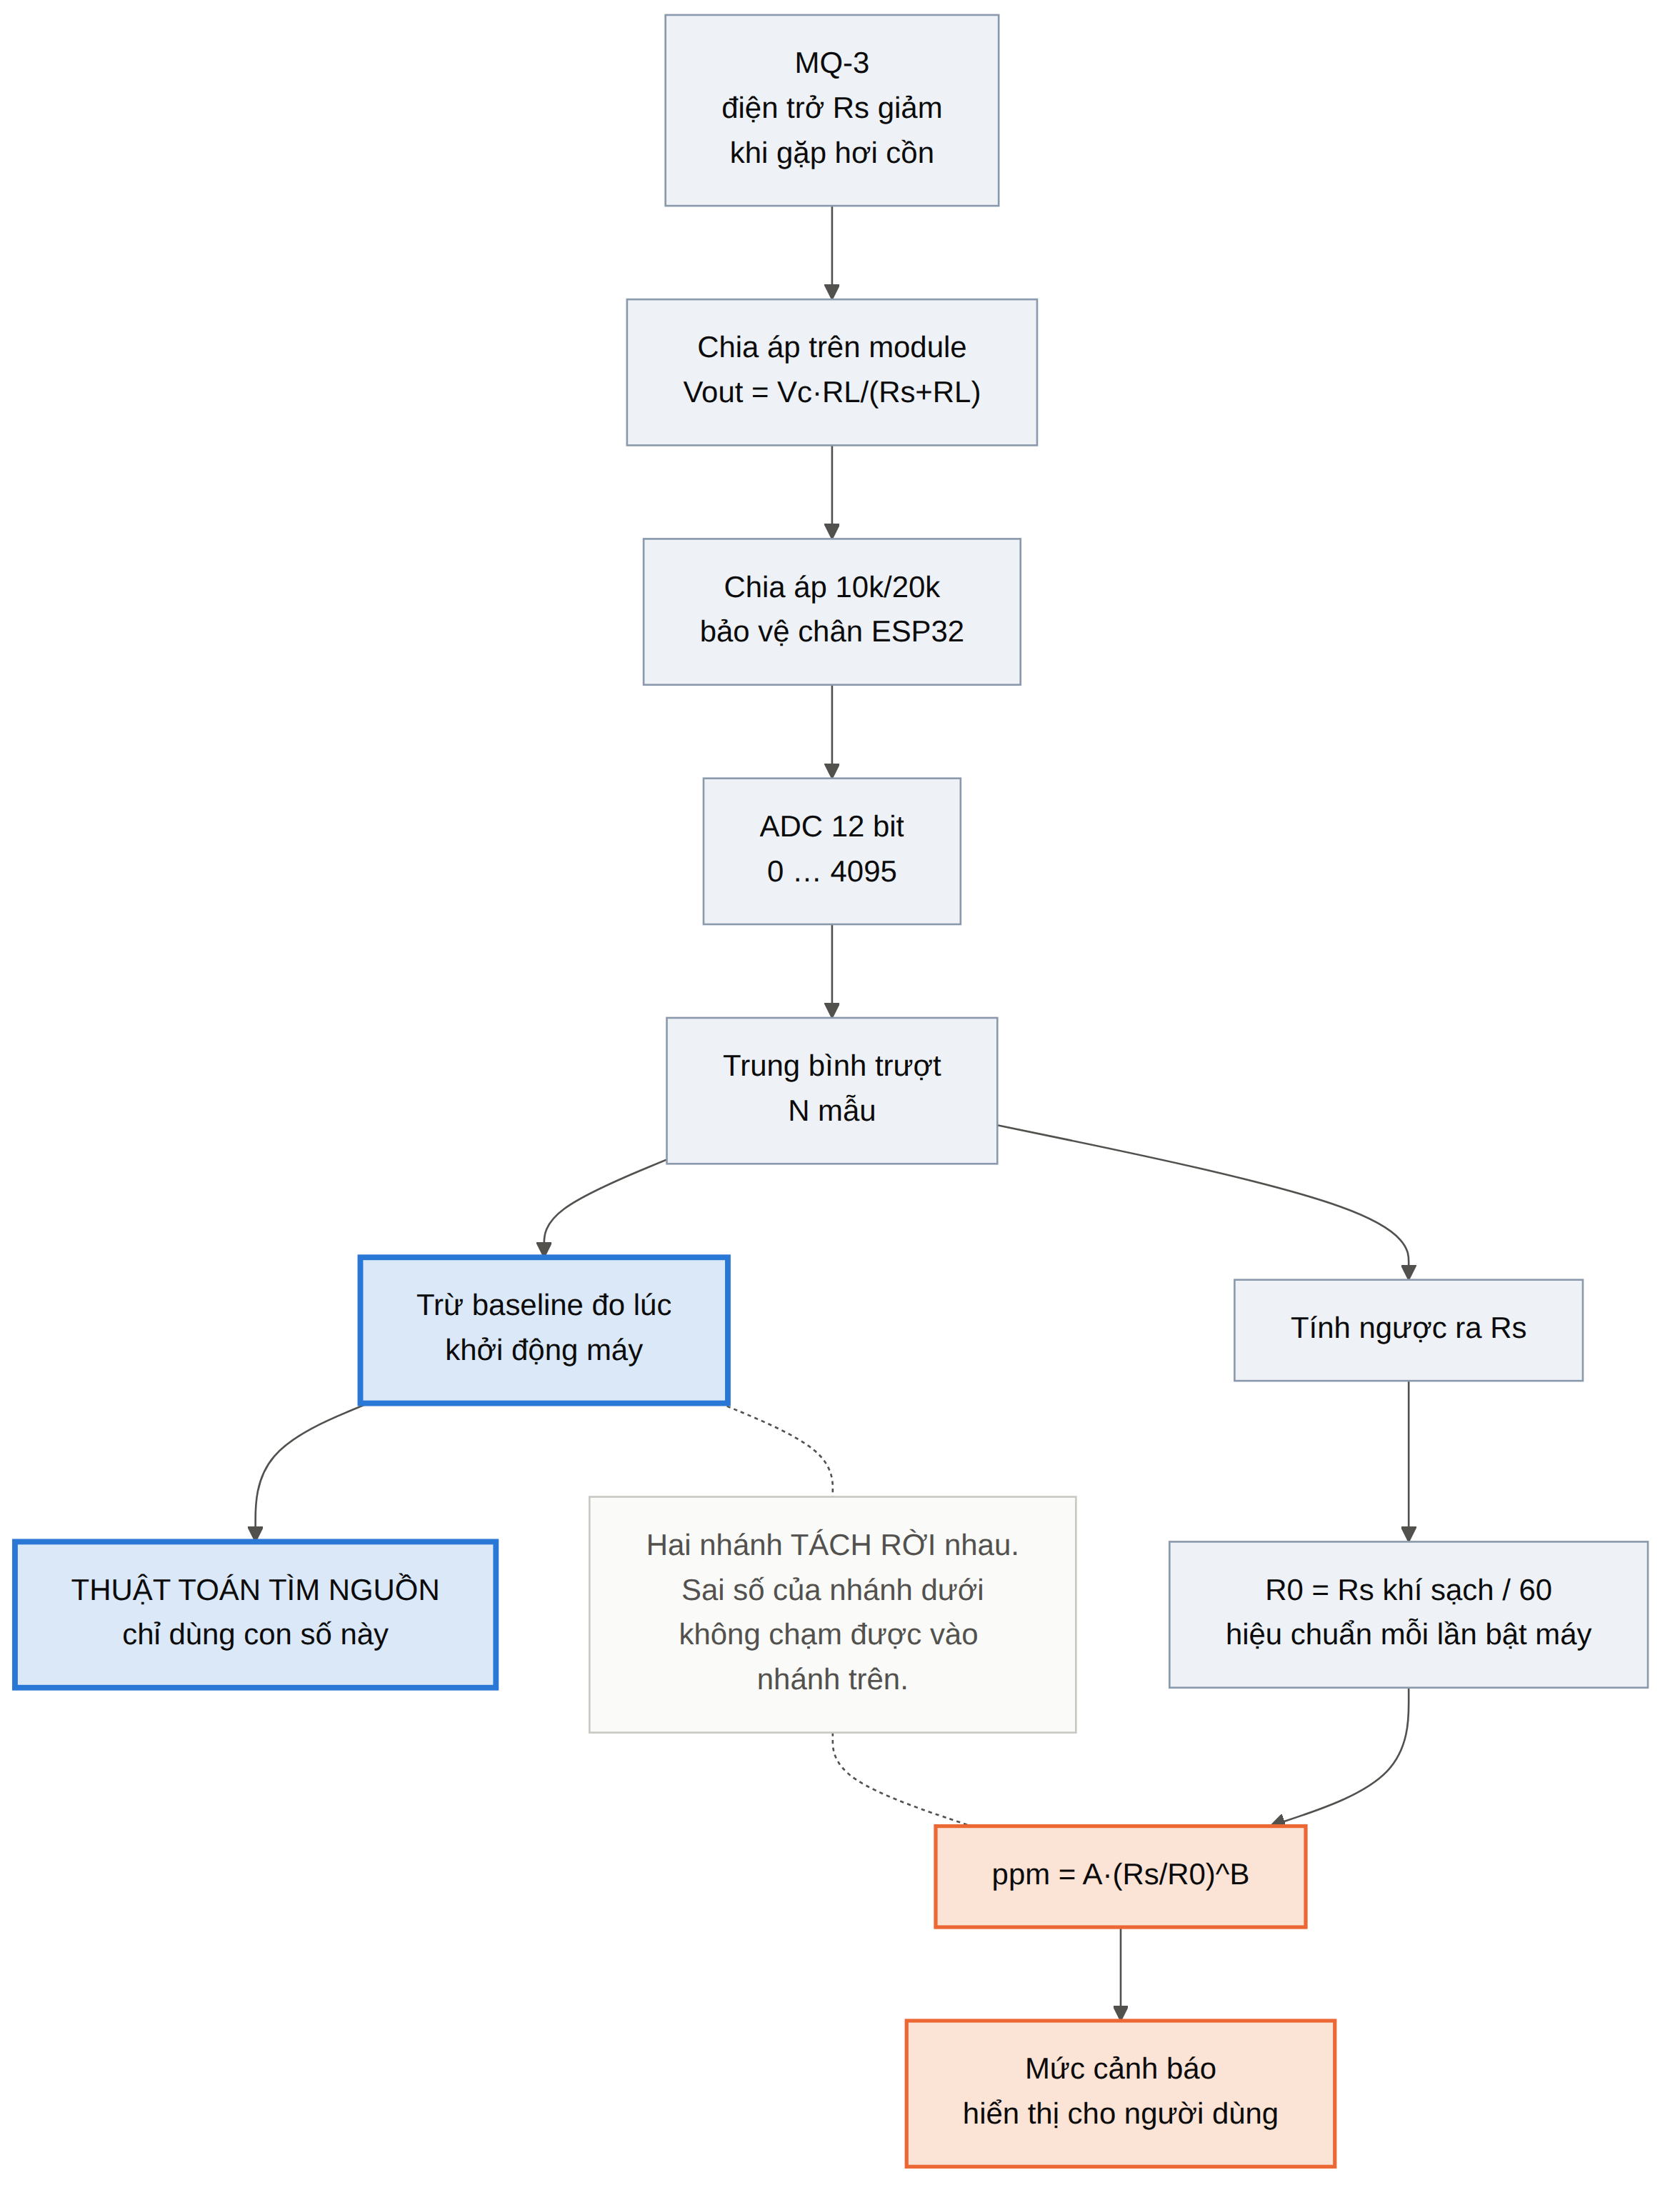
\includegraphics[width=0.941\textwidth]{pic/3_xu_ly_tin_hieu_khi.png}
  \caption{Chuỗi xử lý tín hiệu khí. Hai nhánh tách rời nhau: nhánh trên nuôi thuật toán, nhánh dưới nuôi màn hình hiển thị.}
\end{figure}
Hình 4.1 trình bày toàn bộ chuỗi xử lý. Đây là quyết định thiết kế quan trọng nhất của phần mềm, và nó là hệ quả trực tiếp của hệ số khuếch đại sai số 1,87 đã phân tích ở mục 2.2.3.

Tín hiệu đi vào theo một đường chung: MQ-3 đổi nồng độ thành điện trở $\rightarrow$ mạch chia áp trên module đổi điện trở thành điện áp $\rightarrow$ mạch chia áp 10k/20k hạ điện áp về mức an toàn cho chân ESP32 $\rightarrow$ ADC 12 bit lấy mẫu ở \textbf{20 Hz} $\rightarrow$ \textbf{trung bình trượt 16 mẫu} (cửa sổ khoảng 0,8 giây).

Bộ lọc trung bình trượt có hai vai trò. Nó giảm nhiễu điện ngẫu nhiên theo quy luật căn bậc hai của số mẫu, tức là khoảng 4 lần với 16 mẫu. Và độ trễ nhóm mà nó đưa vào --- khoảng 375 ms --- \textbf{nằm gọn bên trong} 1,5 giây chờ ổn định của quy trình đo trình bày ở mục 4.3, nên không làm chậm thêm phép đo.

Sau bộ lọc, tín hiệu \textbf{tách làm hai nhánh không bao giờ gặp lại nhau}.

\textbf{Nhánh thứ nhất --- tín hiệu điều khiển.} Lấy giá trị ADC đã lọc \textbf{trừ đi giá trị nền đo lúc khởi động} (giai đoạn 5 giây trong không khí sạch). Kết quả là một số nguyên có dấu, đơn vị là đếm ADC. \textbf{Đây là đại lượng duy nhất mà ba thuật toán tìm nguồn được phép sử dụng.}

\textbf{Nhánh thứ hai --- nồng độ ước lượng để hiển thị.} Tính ngược ra Rs, chia cho R$_{0}$ đã tự hiệu chuẩn lúc khởi động, đưa qua đường đặc tuyến luỹ thừa ra giá trị ppm, rồi so với ba ngưỡng cảnh báo 100 / 500 / 1500 ppm để hiển thị bốn mức: An toàn, Đã phát hiện, Cao, Nguy hiểm.

\begin{ghichu}
Đây là điểm cần được nhìn thấy rõ nhất trong toàn bộ thiết kế: \textbf{thuật toán tìm nguồn không hề dùng tới ppm}. Nó chỉ so sánh ``chỗ này đọc cao hơn hay thấp hơn chỗ kia''. Do đó sai số khuếch đại 1,87 lần ảnh hưởng tới \textbf{con số báo cho người vận hành}, chứ không chạm được vào \textbf{quyết định định vị}. Nói cách khác, độ chính xác tuyệt đối của cảm biến là một vấn đề về hiển thị, không phải một vấn đề về thuật toán.
\end{ghichu}
Giá trị nền được đo \textbf{một lần} lúc khởi động và \textbf{không tự trôi theo thời gian}. Một đường nền thích nghi sẽ dần ``nuốt'' mất tín hiệu khi robot ở lâu trong vùng có khí --- đúng lúc tín hiệu quan trọng nhất. Người vận hành có thể yêu cầu đo lại đường nền bằng một lệnh trên cổng nối tiếp nếu điều kiện phòng thay đổi giữa buổi.


\subsection{Quy trình đo ``dừng ngửi''}
\begin{figure}[!p]
  \centering
  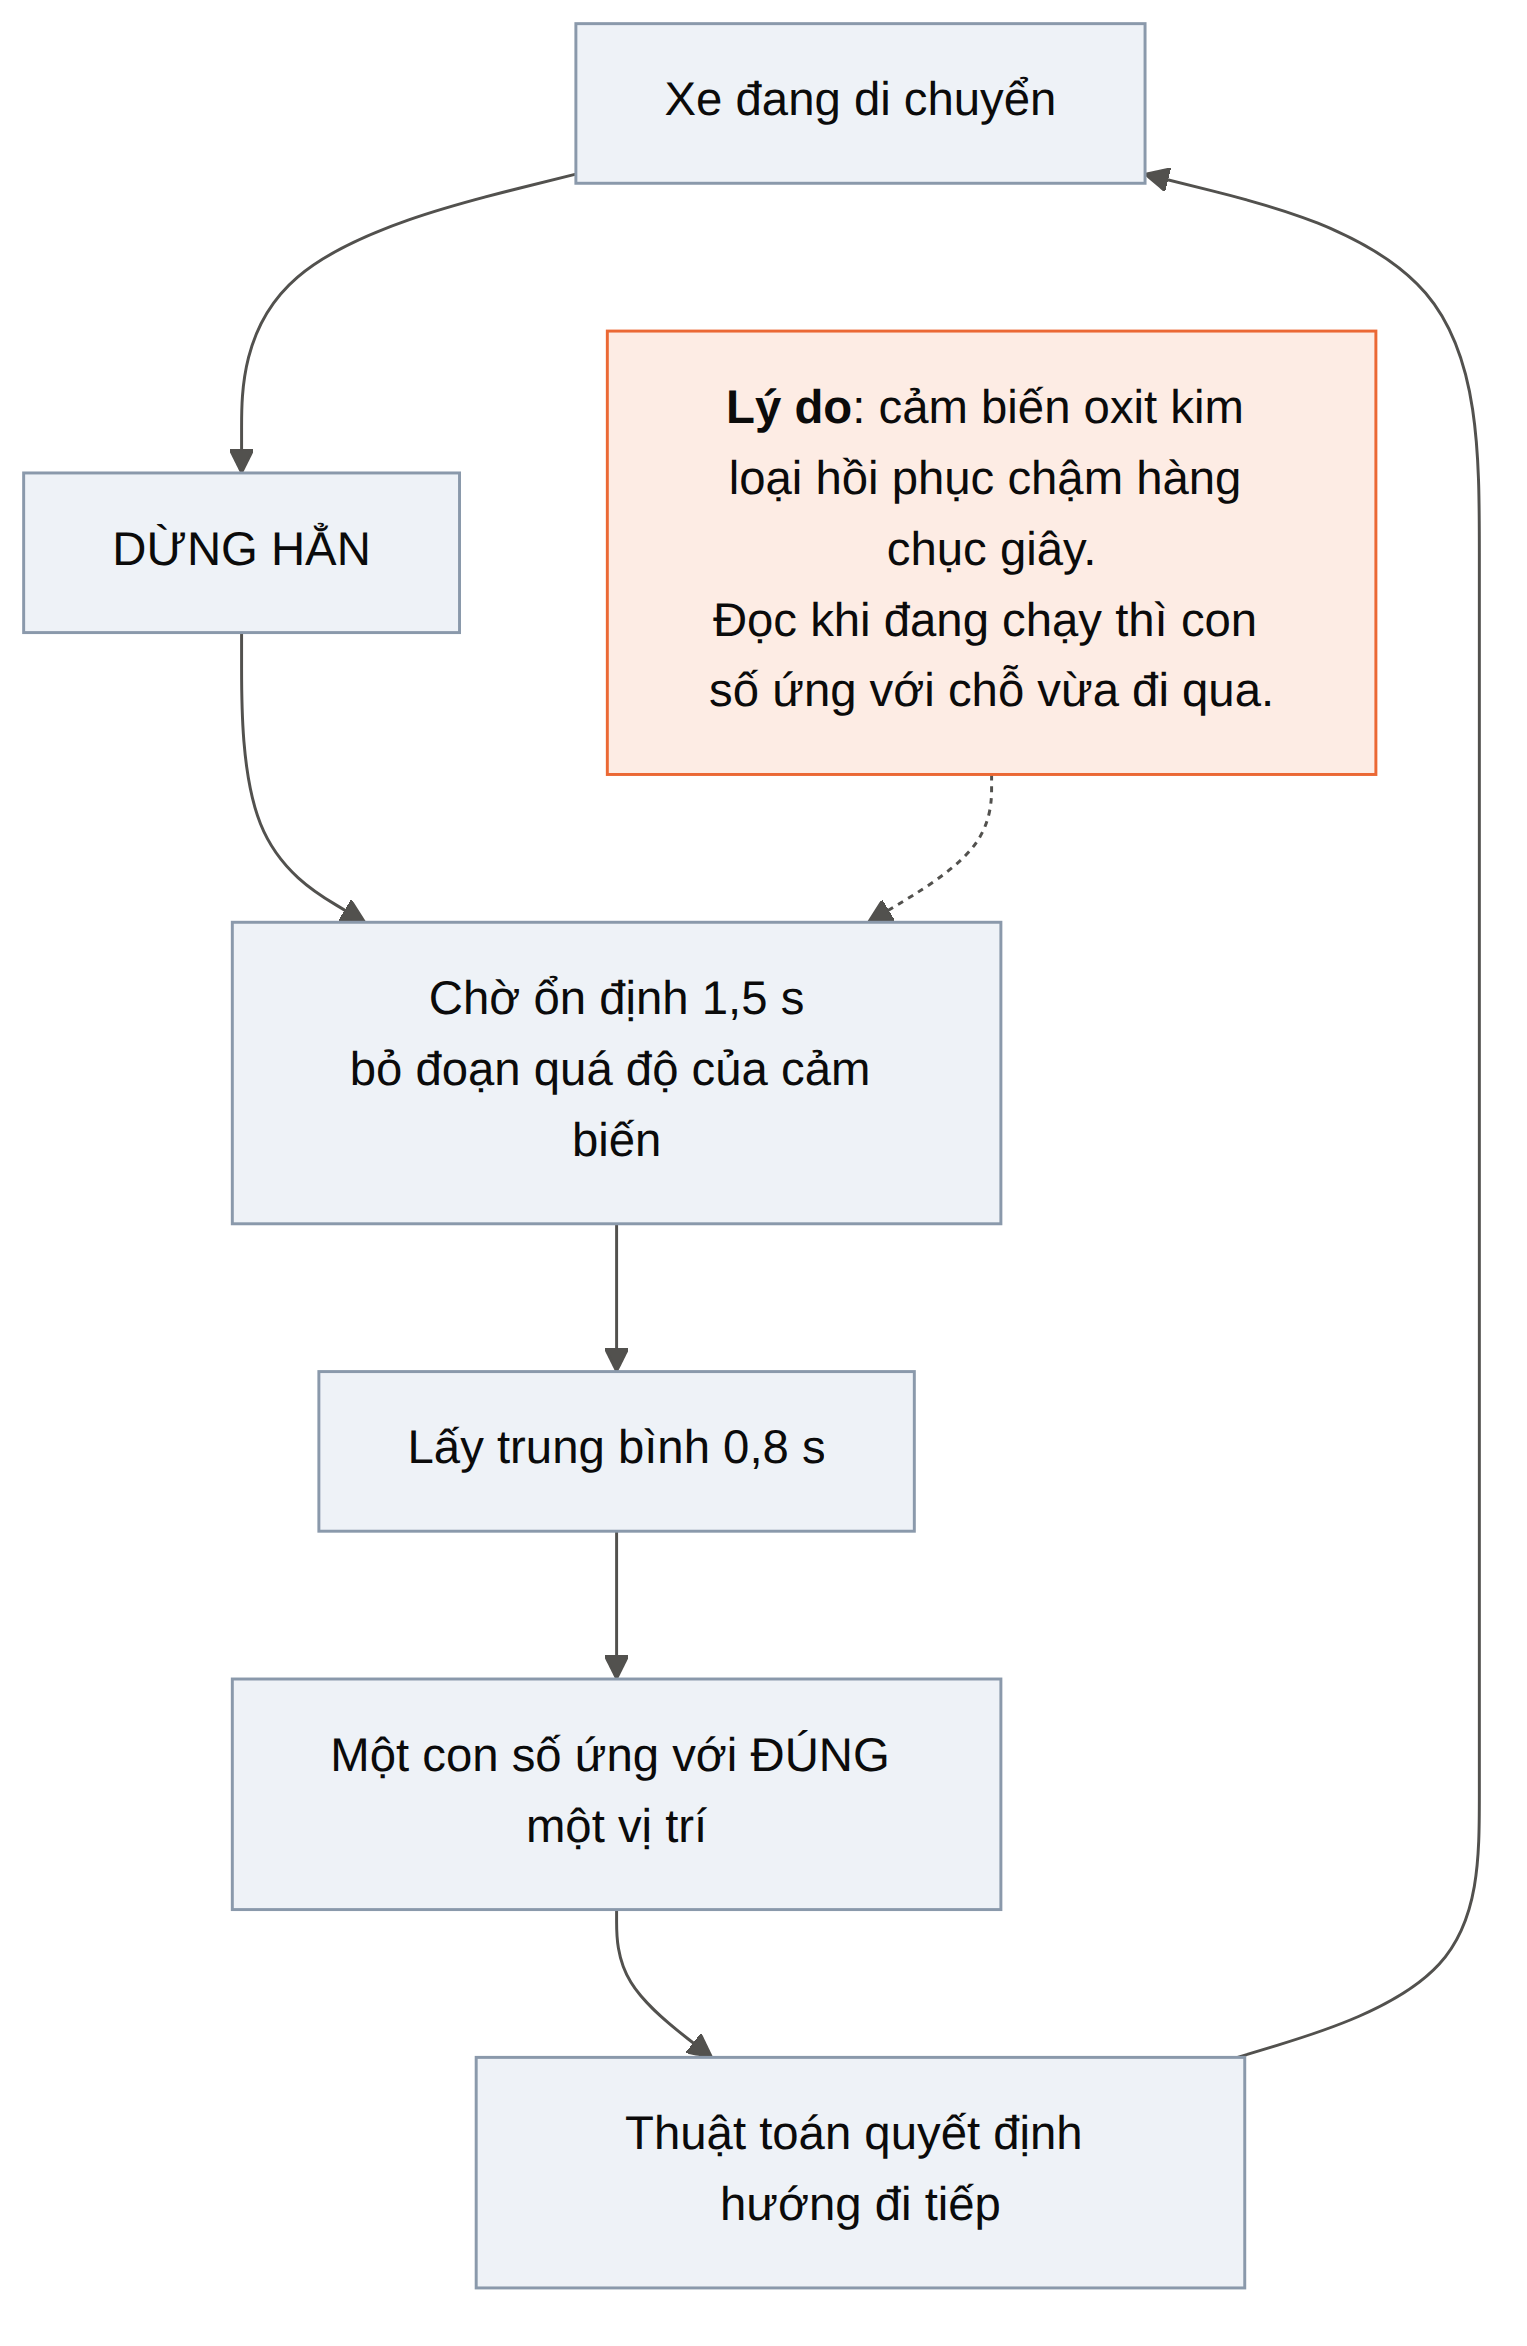
\includegraphics[width=0.859\textwidth]{pic/4_chu_trinh_ngui.png}
  \caption{Chu trình một phép đo. Mọi phép đo đều bắt đầu bằng việc dừng hẳn xe.}
\end{figure}
Từ giới hạn vật lý đã phân tích ở mục 2.3 --- cảm biến MOX hồi phục hàng chục giây và tạo ra ``hiệu ứng đuôi'' dọc đường đi --- nhóm rút ra một quy tắc tuyệt đối, minh hoạ ở Hình 4.2: \textbf{không bao giờ đọc cảm biến trong lúc xe đang chạy.} Mọi phép đo đều theo đúng bốn bước:

\begin{enumerate}[leftmargin=1.6em,itemsep=0.15em,topsep=0.3em]
  \item Xe \textbf{dừng hẳn} và phanh trong 250 ms.
  \item Chờ \textbf{1,5 giây} cho qua đoạn quá độ của cảm biến.
  \item Lấy \textbf{trung bình trong 0,8 giây} tiếp theo.
  \item Kết quả là \textbf{một con số ứng với đúng một vị trí xác định} trong không gian.
\end{enumerate}
Cái giá phải trả rất cụ thể: mỗi phép đo mất \textbf{2,3 giây}, và một lượt quét toàn bộ 64 ô của sân mất khoảng bốn phút. Nhóm chấp nhận cái giá đó, vì nếu không thì mọi con số so sánh về sau đều không có ý nghĩa: chúng sẽ ứng với những vị trí không xác định.


\subsection{Thuật toán 1 --- quét toàn bộ theo lưới}
\begin{figure}[!p]
  \centering
  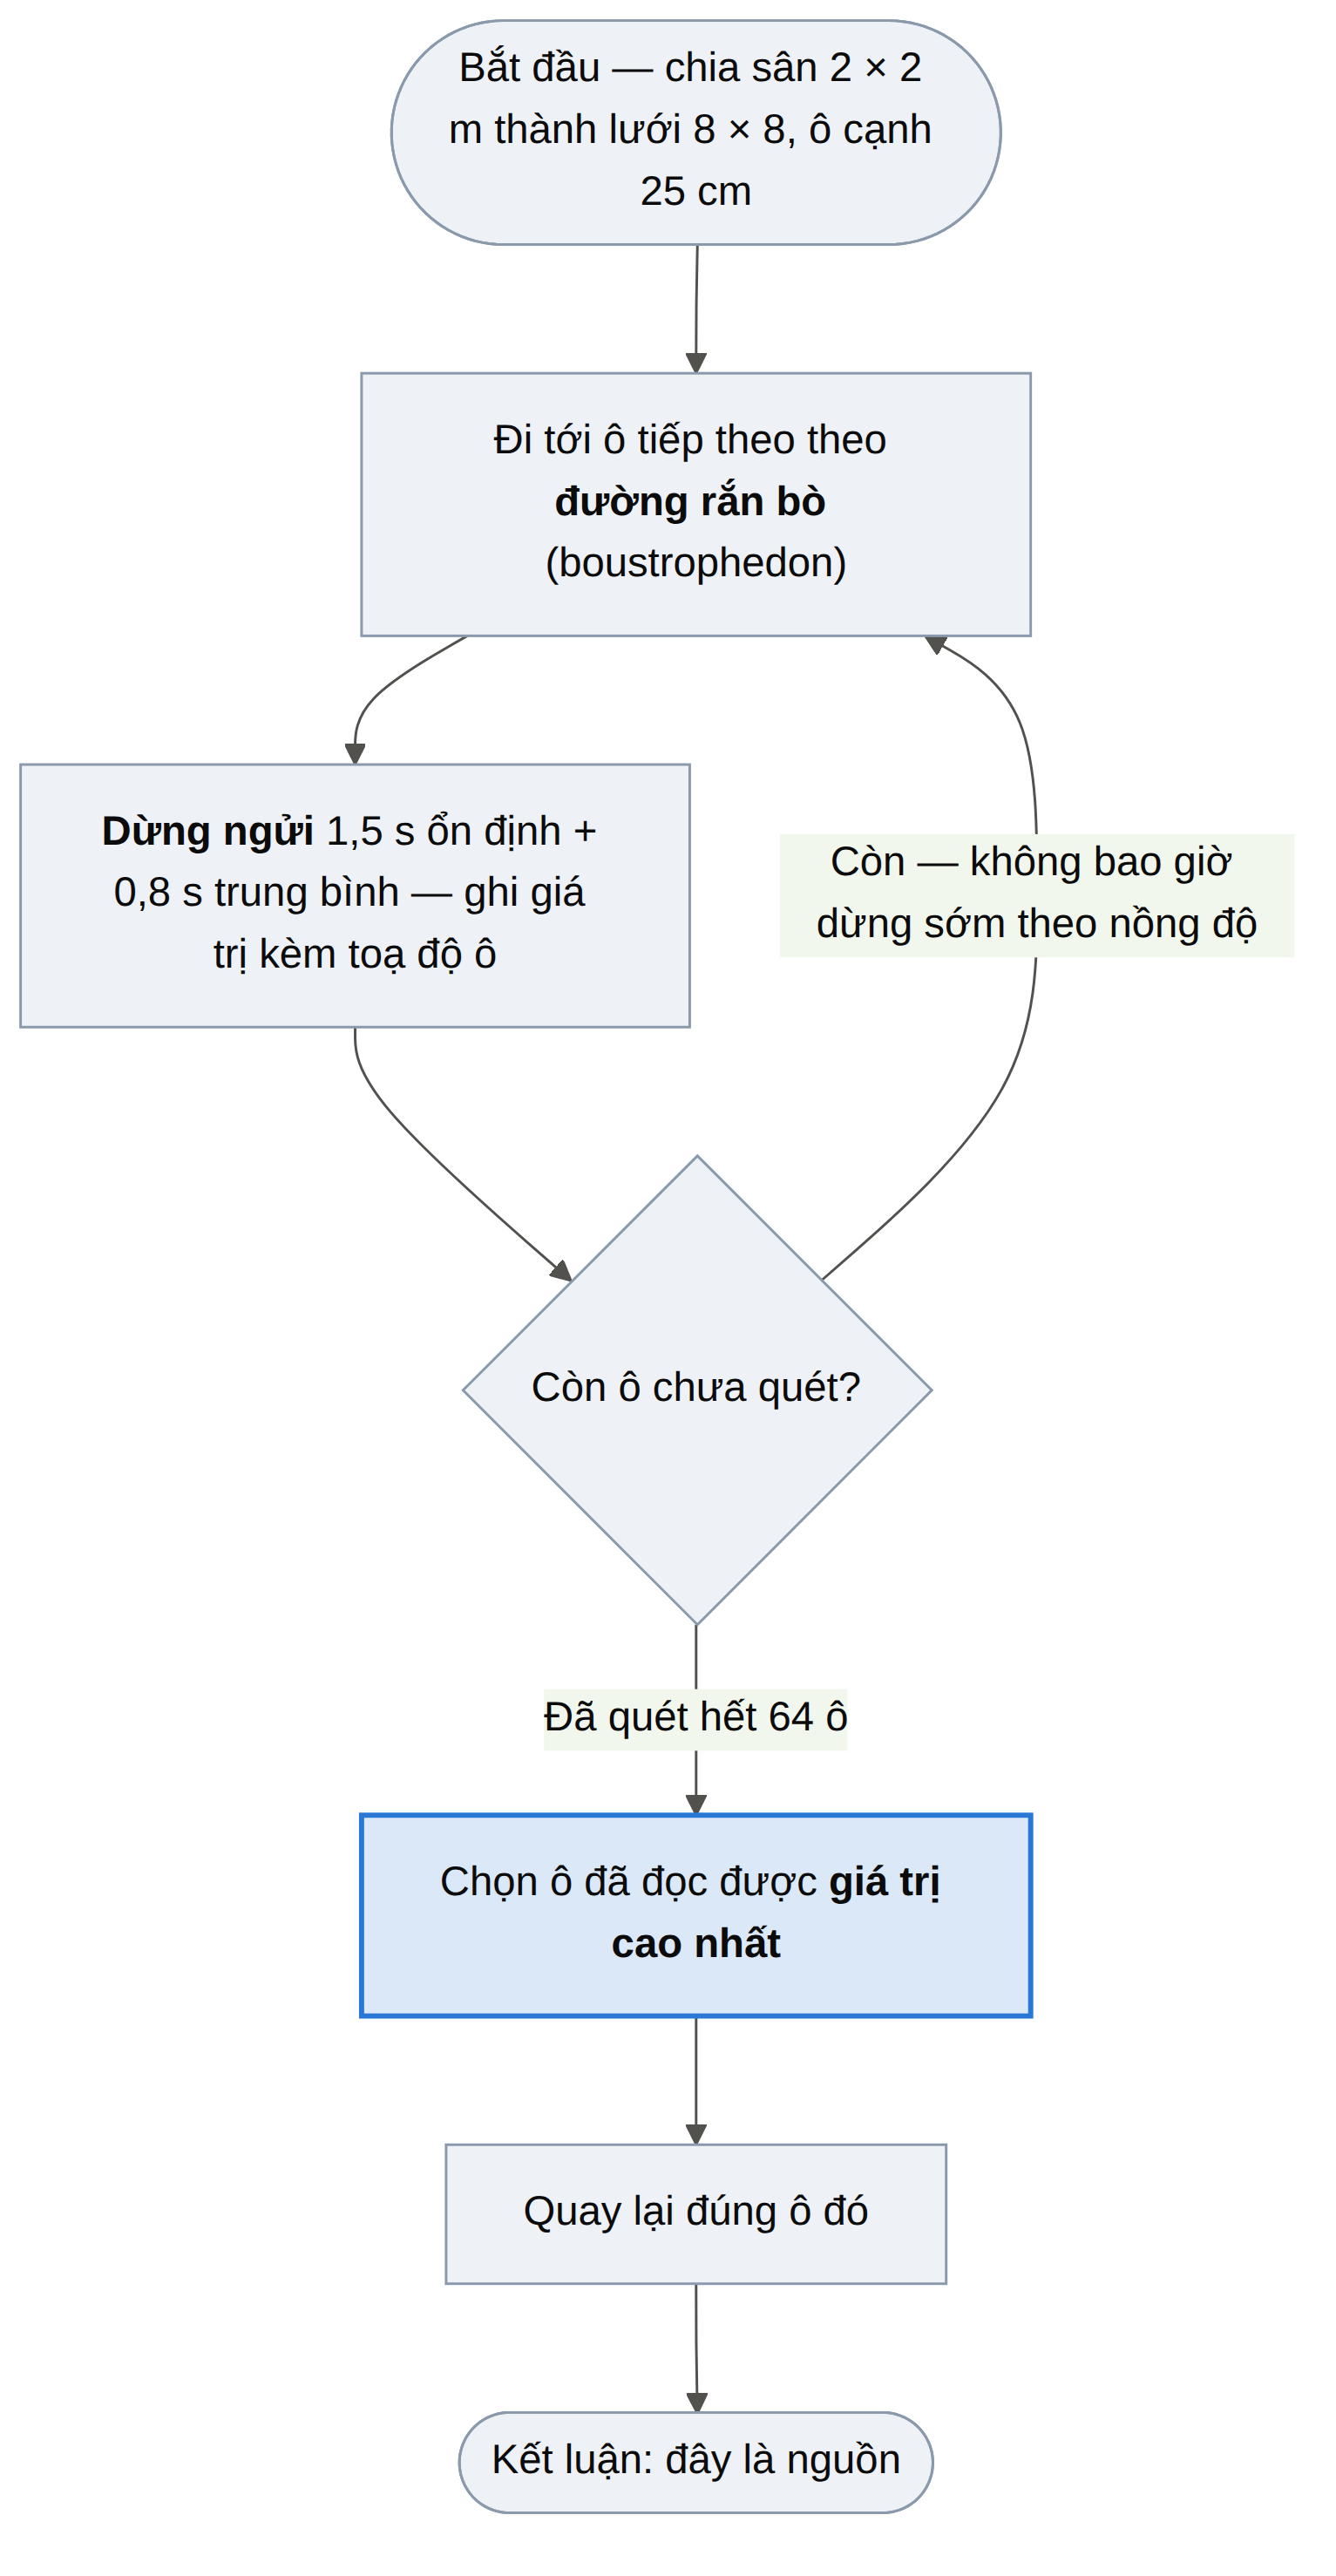
\includegraphics[width=0.684\textwidth]{pic/7_luu_do_quettoanbo.png}
  \caption{Lưu đồ thuật toán quét toàn bộ.}
\end{figure}
Lưu đồ đầy đủ của thuật toán được trình bày ở Hình 4.3. Sân 2 $\times$ 2 m được chia thành lưới 8 $\times$ 8, tổng cộng \textbf{64 ô} cạnh 25 cm. Robot đi hết từng ô theo đường rắn bò, tại mỗi ô thực hiện một phép đo ``dừng ngửi'', ghi lại giá trị và toạ độ. Khi đã quét hết lưới, robot quay lại ô đọc được giá trị cao nhất rồi mới kết luận.

Thời gian lý thuyết ước tính được từ các hằng số của hệ thống: mỗi ô tốn 2,3 giây đo cộng với thời gian di chuyển 25 cm ở tốc độ 18 cm/s, tức khoảng 1,4 giây, tổng cộng khoảng 3,7 giây mỗi ô. Với 64 ô, con số lý thuyết là \textbf{khoảng 236 giây}. Số đo được từ mô phỏng ở Chương 6 là \textbf{273,6 $\pm$ 7,1 giây}. Chênh lệch khoảng 38 giây tương ứng với thời gian quay đầu ở cuối mỗi hàng, thời gian phanh và thời gian quay lại điểm đo cao nhất --- nghĩa là mô hình \textbf{tự nhất quán}, và phần chênh lệch có lời giải thích cụ thể chứ không phải sai số không rõ nguồn gốc.

Một quyết định thiết kế cần được nêu rõ: quét toàn bộ \textbf{cố ý không được phép dừng sớm} khi gặp nồng độ cao. Nó luôn quét hết lưới. Nếu cho phép dừng sớm, nó sẽ không còn là một mốc so sánh ổn định nữa, vì thời gian của nó sẽ phụ thuộc vào việc nguồn nằm ở đầu hay cuối đường quét.


\subsection{Thuật toán 2 --- bám gradient}
\begin{figure}[!p]
  \centering
  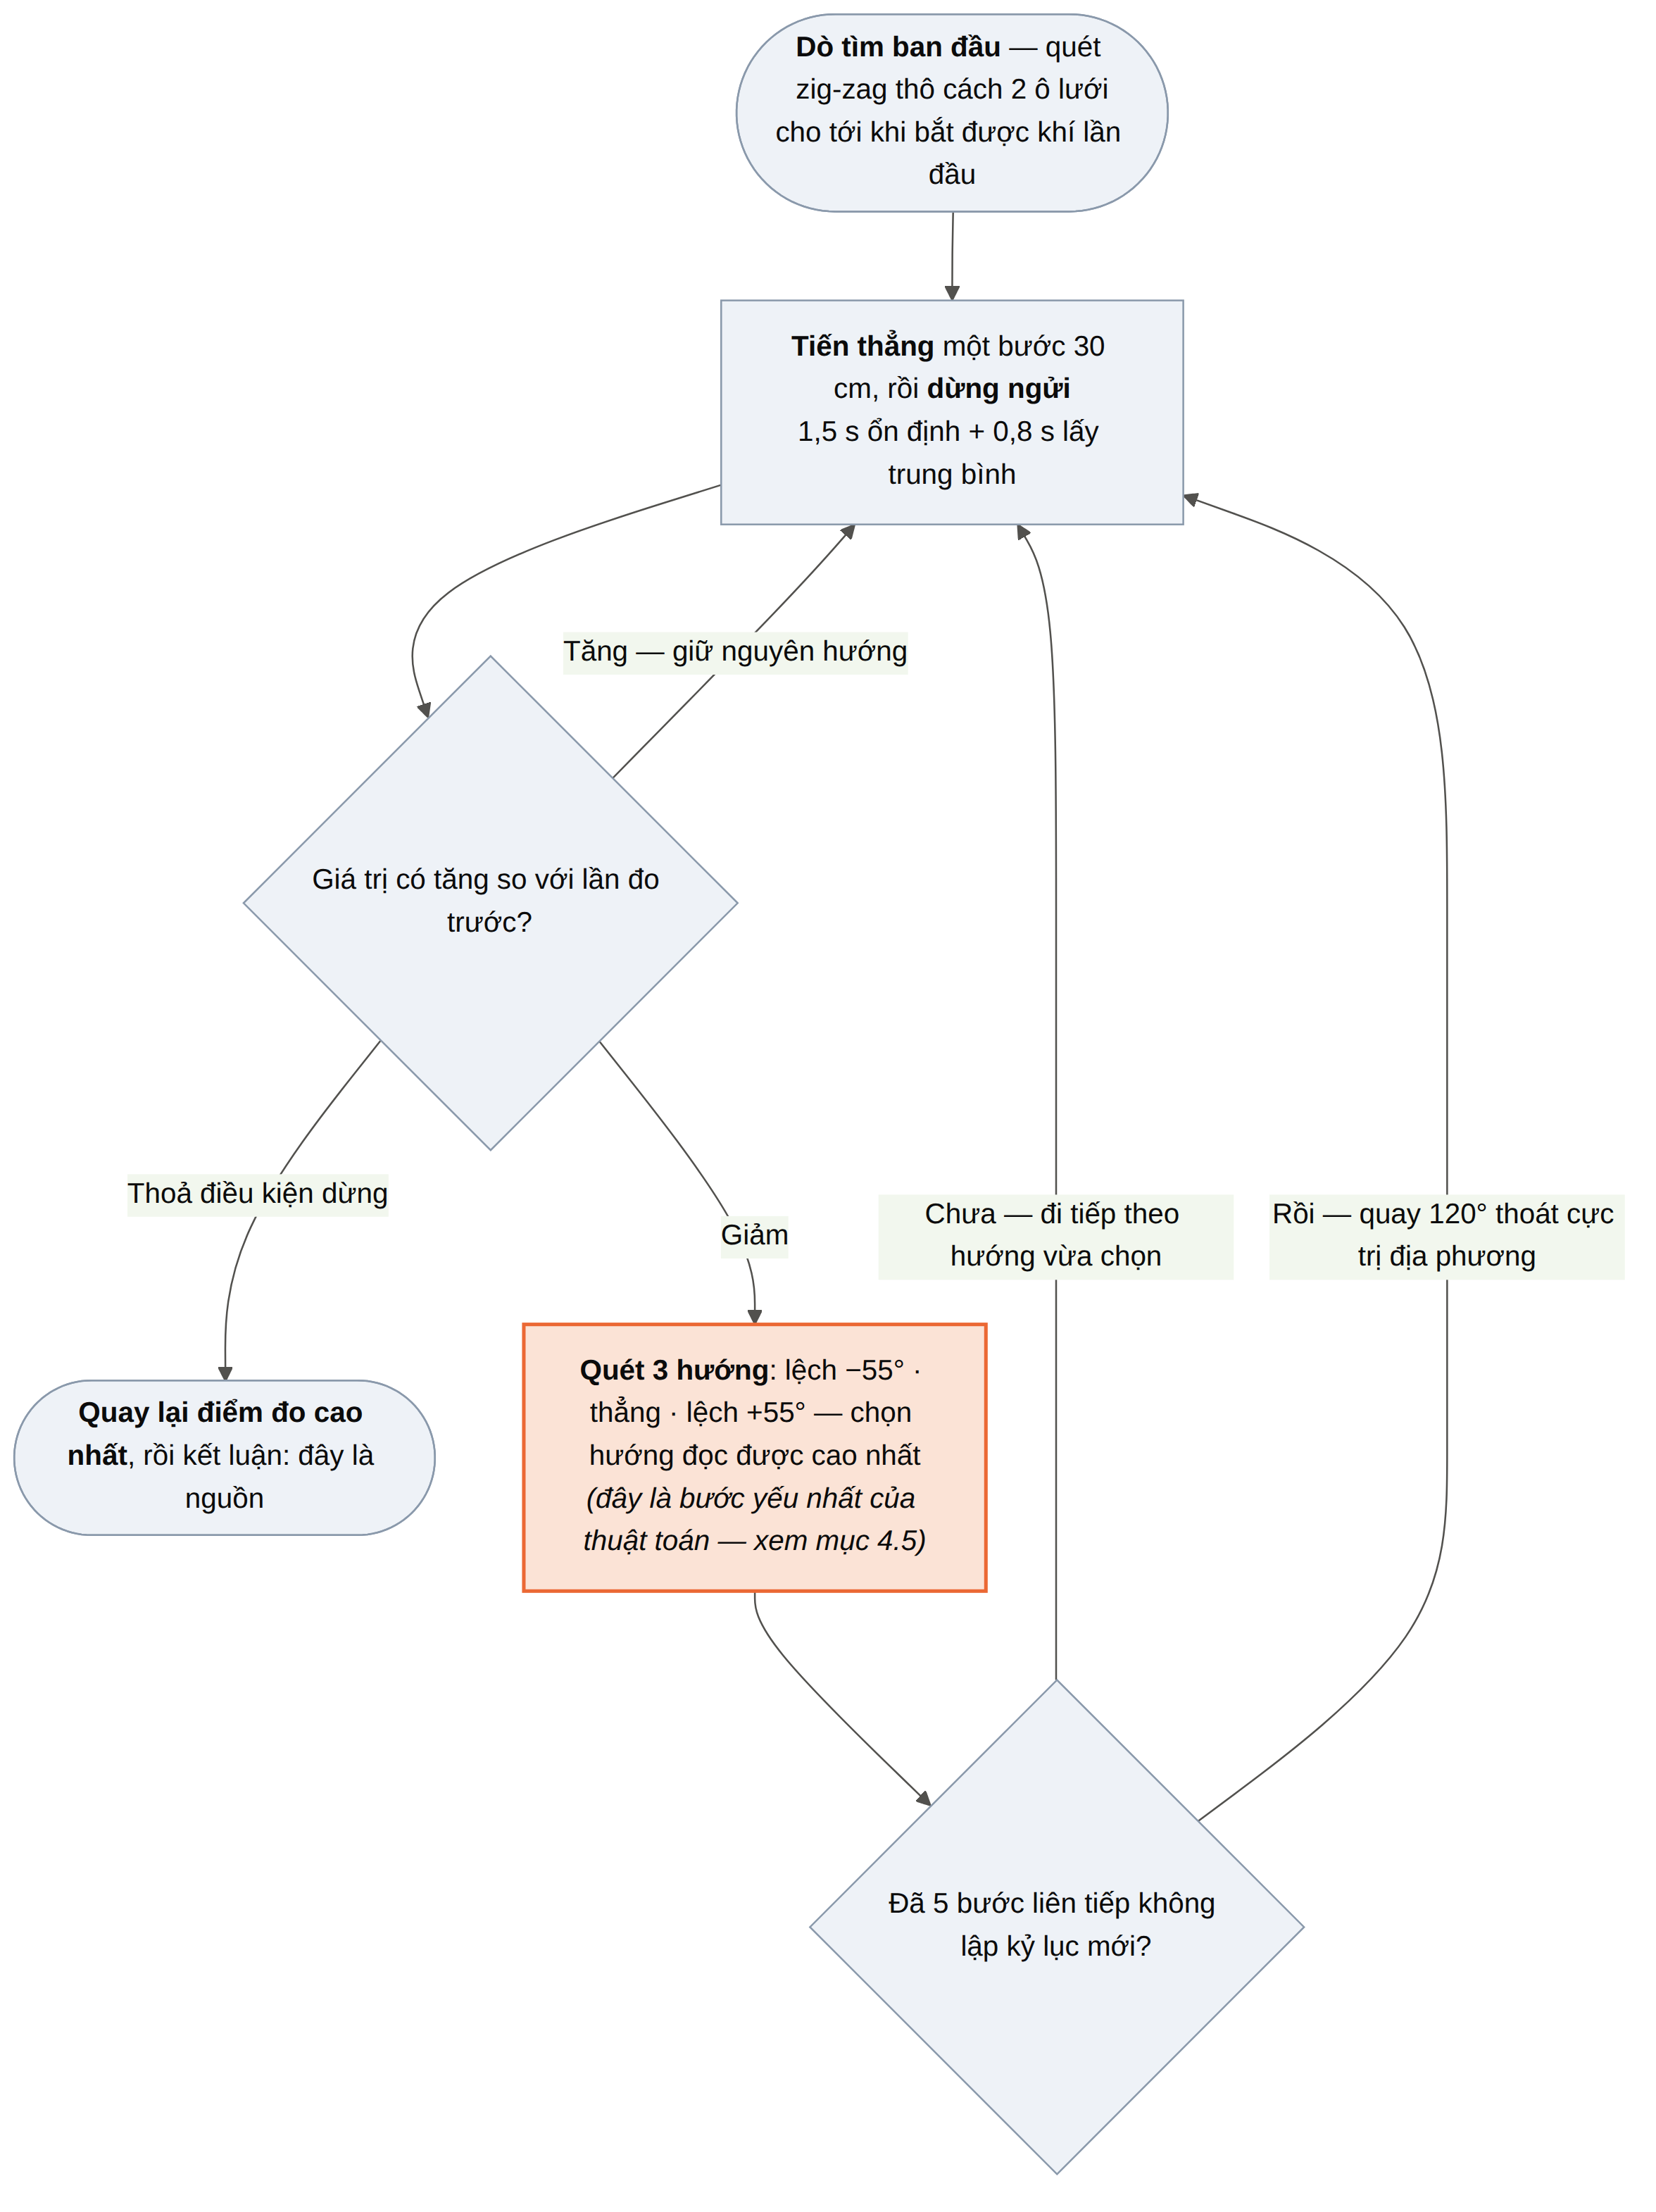
\includegraphics[width=0.941\textwidth]{pic/6_luu_do_gradient.png}
  \caption{Lưu đồ thuật toán bám gradient.}
\end{figure}
Bản cài đặt của nhóm ghép hai biến thể thường gặp trong tài liệu, theo nguyên tắc \textbf{đi thẳng khi giá trị còn tăng, chỉ quét ba hướng khi giá trị giảm}. Vòng lặp điều khiển, tóm tắt ở Hình 4.4, hoạt động như sau.

\begin{enumerate}[leftmargin=1.6em,itemsep=0.15em,topsep=0.3em]
  \item \textbf{Giai đoạn dò tìm ban đầu.} Khi chưa hề phát hiện khí, bám gradient không có gì để bám. Robot quét thô theo đường zig-zag, cách nhau 2 ô lưới, cho tới khi giá trị đọc được vượt ngưỡng phát hiện.
  \item \textbf{Tiến thẳng.} Sau khi bắt được tín hiệu, robot đi thẳng từng bước 30 cm. Sau mỗi bước, nó dừng ngửi một lần và so sánh với giá trị đo trước đó. Chừng nào giá trị \textbf{còn tăng} quá ngưỡng cao nguyên, nó tiếp tục đi thẳng theo đúng hướng cũ.
  \item \textbf{Quét ba hướng.} Khi giá trị \textbf{giảm hoặc không tăng đáng kể}, robot quay lệch \textbf{--55$^\circ$}, đi một bước và đo; rồi quay sang \textbf{+55$^\circ$}, đi một bước và đo. Sau đó nó so sánh ba ứng viên: giá trị vừa đo ở hướng trái, giá trị vừa đo ở hướng phải, và giá trị đã đo trước đó ở hướng thẳng. Hướng nào cao nhất thì trở thành hướng mới.
  \item \textbf{Thoát cực trị địa phương.} Nếu sau 5 bước liên tiếp mà giá trị tốt nhất không được cải thiện, robot coi như đang mắc kẹt tại một cực trị địa phương và \textbf{quay một góc lớn 120$^\circ$} rồi đi tiếp.
  \item \textbf{Kết luận.} Khi thoả điều kiện dừng (mục 4.7), robot quay về điểm đã đo được giá trị cao nhất rồi mới báo kết quả.
\end{enumerate}
\begin{ghichu}
Một chi tiết cần được nêu trung thực vì nó là \textbf{điểm yếu đã biết} của bản cài đặt: trong bước 3, giá trị của ứng viên ``thẳng'' là một giá trị \textbf{đã đo từ trước}, không phải một phép đo mới. Nghĩa là ba con số được so sánh không hoàn toàn cùng thời điểm. Việc ưu tiên đi thẳng ở bước 2 chính là biện pháp giảm thiểu vấn đề này: khi đi thẳng, hai phép đo cách nhau 30 cm, chênh lệch không gian đủ lớn để lấn át phần dư âm của cảm biến. Chỉ khi giá trị thực sự giảm thì mới phải chấp nhận thao tác quét ba hướng, và nhóm biết rằng đó là bước yếu nhất của thuật toán này.
\end{ghichu}

\subsection{Thuật toán 3 --- surge-casting}
\begin{figure}[!htbp]
  \centering
  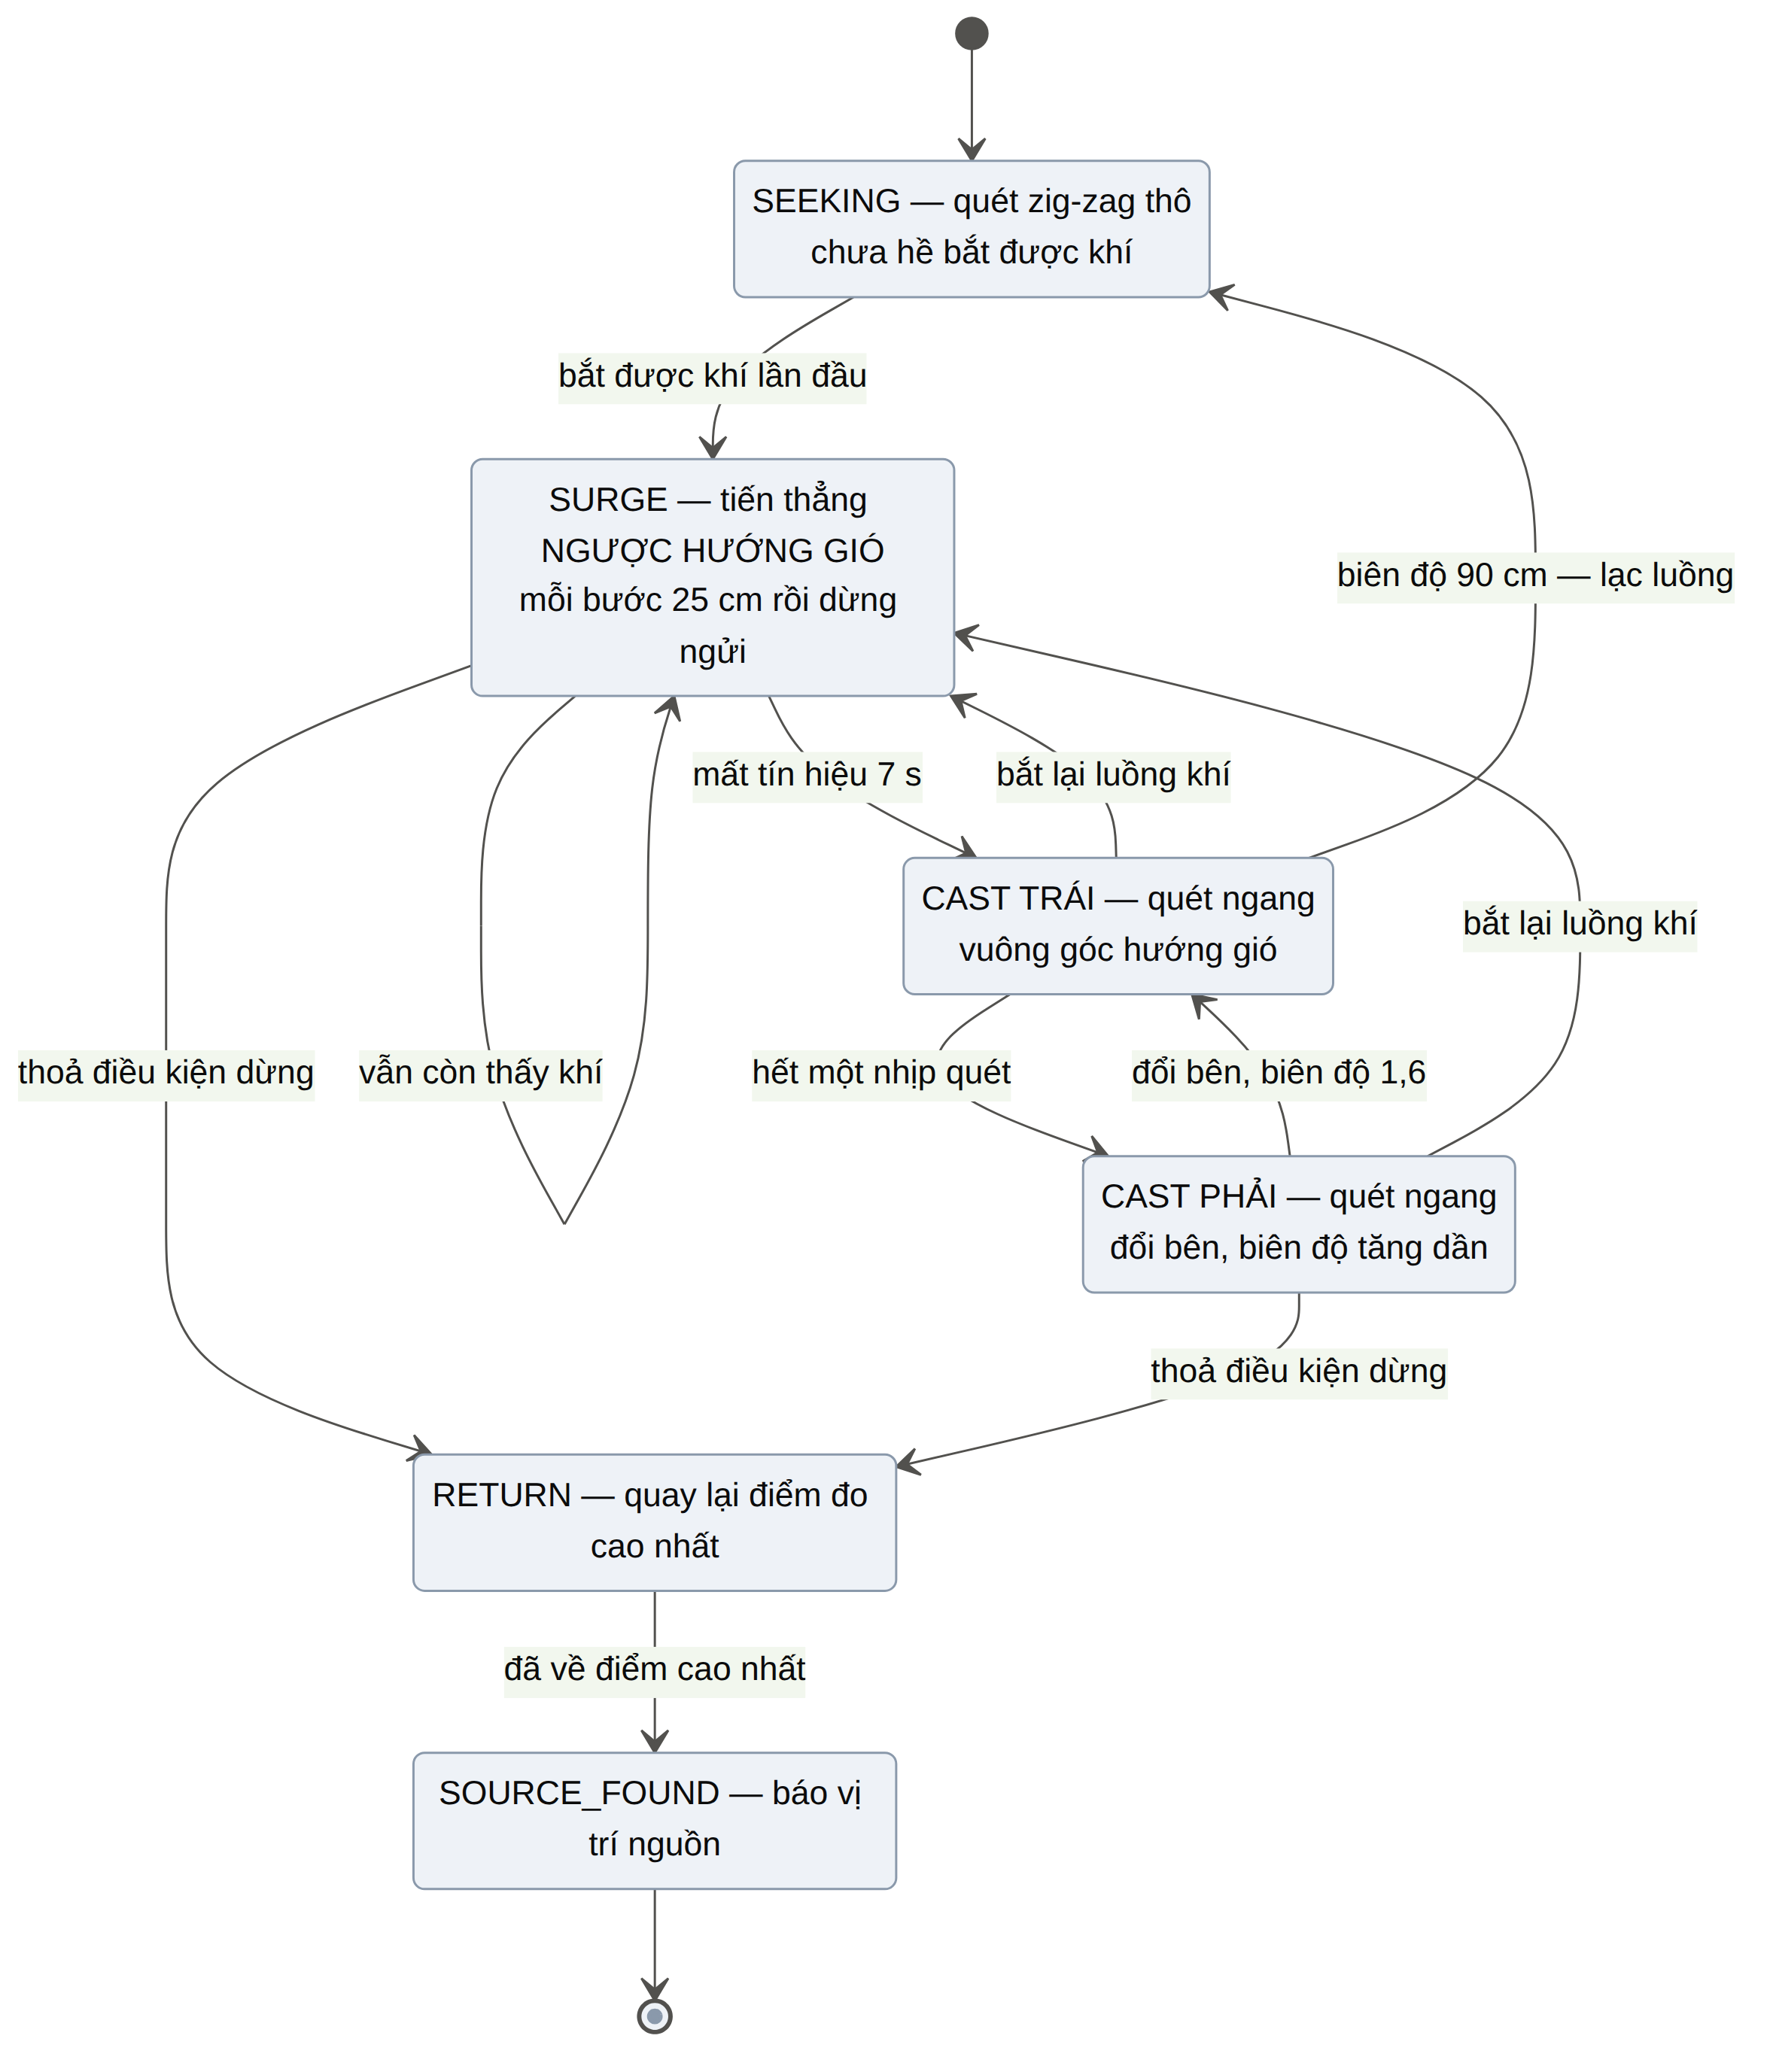
\includegraphics[width=0.941\textwidth]{pic/5_fsm_surgecast.png}
  \caption{Máy trạng thái của thuật toán surge-casting.}
\end{figure}
Surge-casting được cài đặt dưới dạng một \textbf{máy trạng thái hữu hạn} gồm năm trạng thái, trình bày ở Hình 4.5.

\textbf{SEEKING} --- chưa hề ngửi thấy gì. Robot quét thô zig-zag khắp sân, bước đi 30 cm, cách nhau 2 ô lưới. Đây là \textbf{cùng một cơ chế} với giai đoạn dò tìm ban đầu của bám gradient, và điều đó là có chủ ý: nếu để mỗi thuật toán tự xoay xở khi chưa có tín hiệu thì bảng so sánh ở Chương 6 sẽ đo lẫn cả ``khả năng dò mù'' vào kết quả, trong khi H1 và H2 chỉ nói về hành vi \textbf{sau khi} đã bắt được luồng khí.

\textbf{SURGE} --- đang ngửi thấy. Robot tiến từng bước 25 cm \textbf{ngược hướng gió}, mỗi bước dừng ngửi một lần. Còn ngửi thấy thì còn tiến.

\textbf{CAST} --- đã mất tín hiệu quá 7 giây (tương đương khoảng hai chu kỳ đo liên tiếp không thấy khí; khoảng chờ này cho phép robot giữ ``quán tính'' đi xuyên qua một khoảng trống giữa hai cụm khí, đúng như hành vi của côn trùng). Robot quét ngang \textbf{vuông góc hướng gió}, đổi bên sau mỗi nhịp, biên độ bắt đầu từ 15 cm và \textbf{nhân 1,6 lần sau mỗi lần đổi bên}. Biên độ tăng dần là chi tiết bắt buộc: nếu giữ nguyên biên độ, robot sẽ quét đi quét lại đúng một dải hẹp và không bao giờ tìm lại được luồng.

\textbf{Quay lại SURGE} khi bắt lại được tín hiệu. Nếu biên độ cast vượt quá 90 cm mà vẫn không bắt lại được, robot coi như đã lạc hẳn và quay về SEEKING.

\textbf{RETURN} --- khi giá trị không còn cải thiện nữa, robot quay lại \textbf{điểm đã đo được giá trị cao nhất} rồi mới báo kết luận.

\textbf{Giới hạn cần nói rõ:} surge-casting cần biết hướng gió, và \textbf{trong phiên bản này robot không tự đo hướng gió}. Quạt được đặt cố định ở một cạnh sân và hướng gió là một điều kiện biên khai báo trước cho firmware. Hướng khắc phục đã được xác định: gắn thêm một cánh gió hoặc một cảm biến gió kiểu dây nhiệt. Máy trạng thái \textbf{không phải sửa gì cả}, vì nó chỉ đọc một biến ``hướng gió'' --- hiện tại biến đó là hằng số, sau này nó là giá trị đọc từ cảm biến.


\subsection{Các cơ chế dùng chung cho cả ba thuật toán}
Để so sánh công bằng, ba thuật toán dùng chung bốn cơ chế sau.

\textbf{Điều kiện dừng.} Robot chỉ kết luận ``đã tìm thấy nguồn'' khi thoả \textbf{đồng thời} cả ba điều kiện: (i) giá trị chuẩn hoá vượt ngưỡng cao; (ii) giá trị không tăng quá ngưỡng cao nguyên so với giá trị tốt nhất trước đó; và (iii) hai điều kiện trên được duy trì liên tục trong 6 giây, tương đương khoảng hai chu kỳ đo liên tiếp không cải thiện. Điều kiện thứ ba là cần thiết vì nếu không, một lần đọc nhiễu đơn lẻ cũng đủ làm robot dừng sớm.

\textbf{Quay lại điểm tốt nhất.} Do độ trễ của cảm biến, robot hầu như luôn \textbf{đi quá đỉnh rồi mới nhận ra}. Vì vậy cả ba thuật toán, khi thoả điều kiện dừng, đều quay lại điểm đã đo được giá trị cao nhất rồi mới báo kết quả. Đây không phải một chi tiết phụ: nhóm đã chạy lại \textbf{toàn bộ 180 lần chạy với đúng bộ hạt giống cũ} nhưng tắt cơ chế này, và kết quả sụp đổ. Sai số trung bình của quét toàn bộ trong môi trường khuếch tán tăng từ 22,7 cm lên \textbf{148,1 cm}, tỉ lệ thành công rơi từ 23/30 xuống \textbf{0/30}; bám gradient trong cùng môi trường tăng từ 26,0 cm lên \textbf{74,0 cm}, tỉ lệ thành công từ 20/30 xuống \textbf{0/30}. Nói cách khác, nếu robot kết luận ngay tại chỗ nó đang đứng thì \textbf{gần như không bao giờ dừng được trong phạm vi 30 cm quanh nguồn} --- nó luôn đã đi quá. Thời gian quay lại \textbf{được tính vào tổng thời gian} trong bảng kết quả; nhóm không giấu chi phí này đi.

\textbf{Chống kẹt.} Nếu sau 12 phép đo liên tiếp mà không lập được kỷ lục mới, robot kết luận bằng điểm cao nhất đã đo được thay vì lang thang cho tới hết giờ. Không có cơ chế này, surge-casting từng kẹt trong một vòng lặp vô hạn ở góc sân: không tiến ngược gió được nên chuyển sang cast, cast lại phát hiện khí nên đặt lại biên độ, rồi lặp mãi. Bộ đếm chống kẹt chỉ được đặt lại khi giá trị \textbf{vượt kỷ lục cũ quá ngưỡng cao nguyên}, chứ không phải mỗi khi có một giá trị cao hơn dù chỉ một đếm ADC --- nếu không, trong trường nhiễu nó gần như không bao giờ kích hoạt.

\textbf{Phản ứng va chạm.} Khi công tắc va chạm đóng, robot lùi 12 cm rồi quay $\pm$75$^\circ$, đổi bên sau mỗi lần. Một ngoại lệ quan trọng: \textbf{trong pha quay lại điểm tốt nhất, va chạm làm robot dừng hẳn tại chỗ} và giữ nguyên kết luận đã ghi. Nếu không có ngoại lệ này, robot sẽ rơi vào vòng lặp kết luận $\leftrightarrow$ tìm lại cho tới hết giờ --- một lỗi mà cả ba thuật toán đều từng mắc và được bộ kiểm thử tự động phát hiện.

\begin{table}[!htbp]
  \centering
  \caption{Các hằng số điều khiển chính của ba thuật toán}
  \small
  \renewcommand{\arraystretch}{1.25}
  \begin{tabular}{>{\raggedright\arraybackslash}p{0.3071\textwidth}>{\raggedright\arraybackslash}p{0.1626\textwidth}>{\raggedright\arraybackslash}p{0.4335\textwidth}}
    \toprule
    \textbf{Hằng số} & \textbf{Giá trị} & \textbf{Ý nghĩa} \\
    \midrule
    Chu kỳ lấy mẫu khí & 50 ms (20 Hz) & Tần số đọc ADC \\
    Cửa sổ trung bình trượt & 16 mẫu ($\approx$ 0,8 s) & Lọc nhiễu điện \\
    Thời gian đo nền & 5 s & Đo trong không khí sạch lúc khởi động \\
    Chờ ổn định khi ngửi & 1 500 ms & Bỏ qua đoạn quá độ của cảm biến \\
    Lấy trung bình khi ngửi & 800 ms & Tổng một phép đo: 2,3 s \\
    Ngưỡng phát hiện khí & 40 đếm ADC & \textbf{Cần đo lại trên phần cứng thật} \\
    Ngưỡng đủ cao để xét dừng & 800 đếm ADC & \textbf{Cần đo lại trên phần cứng thật} \\
    Ngưỡng cao nguyên & 30 đếm ADC & Mức tăng dưới ngưỡng này coi là ``không tăng'' \\
    Thời gian giữ điều kiện dừng & 6 000 ms & $\approx$ 2 chu kỳ đo không cải thiện \\
    Bước tiến của bám gradient & 30 cm &  \\
    Góc quét của bám gradient & $\pm$55$^\circ$ & Cho khoảng cách đầu dò hiệu dụng $\approx$ 20 cm \\
    Số bước không cải thiện để thoát & 5 & Rồi quay 120$^\circ$ \\
    Bước tiến ngược gió (surge) & 25 cm &  \\
    Thời gian mất tín hiệu để cast & 7 000 ms &  \\
    Biên độ cast ban đầu & 15 cm & Nhân 1,6 sau mỗi lần đổi bên, tối đa 90 cm \\
    Giới hạn chống kẹt & 12 phép đo & Không lập kỷ lục mới thì kết luận \\
    Thời gian tối đa một lần chạy & 480 s & Tự động dừng để bảo vệ pin \\
    \bottomrule
  \end{tabular}
\end{table}
Bảng 4.2 tập hợp toàn bộ các hằng số điều khiển. Cần ghi nhận rõ: ba ngưỡng đánh dấu ``cần đo lại'' trong bảng này hiện \textbf{vẫn là giá trị phỏng đoán} dựa trên mô hình cảm biến, chưa phải giá trị đo trên phần cứng thật. Đây là một hạn chế được nêu lại ở mục 7.2.


\subsection{Giao thức telemetry và trạm mặt đất}
Mỗi giây, xe gửi về trạm một gói tin chứa: nhãn thời gian, thuật toán đang chạy, trạng thái hiện tại của máy trạng thái, vị trí ước lượng, hướng, giá trị ADC thô, giá trị chuẩn hoá, nồng độ ước lượng, mức cảnh báo và mã kiểm tra XOR. Trạm mặt đất kiểm tra mã kiểm tra, in ra một dòng máy đọc để một chương trình Python ghi thành tệp CSV, và một dòng người đọc để theo dõi trực tiếp.

Đường lệnh ngược từ trạm lên xe được giữ lại với hai lệnh: chạy/dừng từ xa và \textbf{dừng khẩn cấp}. Robot vẫn chạy hoàn toàn độc lập nếu mất sóng.


\subsection{Chế độ kiểm tra phần cứng và bộ kiểm thử tự động}
Firmware có một \textbf{chế độ kiểm tra phần cứng} riêng, tách hẳn khỏi đường chạy thuật toán, gồm các lệnh gõ được qua cổng nối tiếp để: chạy từng động cơ, đi một quãng đường xác định, quay một góc xác định, đọc encoder, đọc công tắc va chạm, in bảng giá trị khí theo thời gian, thực hiện một phép ``dừng ngửi'' đơn lẻ, và thử đường truyền LoRa. Lệnh tự kiểm tra tổng thể lần lượt kiểm tra I$^{2}$C, con quay lúc đứng yên, ADC của MQ-3, công tắc va chạm, LoRa, rồi quay \textbf{từng bánh một} và đếm xung encoder --- nhờ đó phát hiện được cả trường hợp hai dây encoder bị cắm lẫn.

Bộ kiểm thử tự động gồm \textbf{86 phép kiểm tra} chạy trên máy tính trong khoảng một giây, dùng lại robot ảo của trình mô phỏng làm robot giả. Nhóm kiểm tra quan trọng nhất chạy cả ba thuật toán trên 24 tình huống (3 thuật toán $\times$ 2 môi trường $\times$ 4 hạt giống) và \textbf{bắt buộc mọi lần chạy đều phải kết thúc}. Chính bộ kiểm thử này đã phát hiện hai lỗi thật mà mười lần chạy mô phỏng trước đó không thấy: lỗi đặt lại sai bộ đếm chống kẹt, và lỗi pha quay lại điểm tốt nhất bị phản ứng va chạm phá vỡ. Cả hai đã được mô tả ở mục 4.7.
